\documentclass[conference]{IEEEtran}
\IEEEoverridecommandlockouts

\usepackage{amsmath}
\usepackage{amsfonts}
\usepackage{amssymb}
\usepackage{graphicx}
\usepackage{caption}
\usepackage{algorithm}
\usepackage{algorithmic}
\usepackage{booktabs}
\usepackage[colorlinks, citecolor=blue]{hyperref}
\usepackage{xcolor}

\newtheorem{definition}{Definition}

\title{Dynamic Partial Repartitioning of DAG Workflows After Resource Failures
in Federated Fog Environments}

\author{
\IEEEauthorblockN{Gayani Gupta\IEEEauthorrefmark{1},
Mohsen Amini Salehi\IEEEauthorrefmark{1},
Sanjukta Bhowmick\IEEEauthorrefmark{1}}
\IEEEauthorblockA{\IEEEauthorrefmark{1}Dept.\ of Computer Science and
Engineering, University of North Texas, USA \\
\{gayani.gupta, mohsen.aminisalehi, sanjukta.bhowmick\}@unt.edu}
}

\begin{document}
\maketitle

\begin{abstract}
Workflows executed on federated fog infrastructures are commonly modeled as
task DAGs partitioned across heterogeneous, failure-prone resources. When a
fog resource fails mid-execution, the standard remedy---repartitioning and
rescheduling the entire workflow---stalls correct work, migrates healthy
tasks, and inflates communication and recovery cost. We propose a
\emph{dependency-aware partial repartitioning} method that maps a resource
failure in the infrastructure graph to the smallest consistent region of the
task DAG, repartitions only that region onto shortlisted replacement
resources, and incrementally repairs only the communication paths affected by
the failure. We evaluate the method in a custom discrete-event simulator
against full repartitioning, greedy reallocation, a static backup plan, an
exact branch-and-bound solver, and a MILP model solved with HiGHS. Across 120
scenarios, partial repartitioning considers $6\times$ fewer tasks than full
repartitioning, moves $3\times$ fewer tasks, and reduces communication cost by
an order of magnitude, while retaining a makespan within $8\%$ of full
repartitioning and within $0.1\%$ of the exact optimum on small instances. As
workflow size grows, the replanned region stays proportional to the failure's
blast radius---about $10\times$ smaller than full repartitioning at 150
tasks---and under cascaded failures the advantage in both movement and
replanning scope grows further.
\end{abstract}

\section{Introduction}

Federated fog environments distribute workflow tasks across heterogeneous
resources owned by different administrative domains. A workflow is a directed
acyclic graph (DAG): nodes are tasks, edges are data dependencies. The
scheduler partitions the DAG and assigns partitions to fog resources subject
to capacity, memory, communication cost, and deadline constraints.

Resource failures during execution are routine in fog federations. When a
resource fails, unfinished tasks assigned to it can no longer proceed. The
naive remedy---repartitioning and rescheduling the whole workflow---is
expensive three ways: (i)~it must be computed quickly while the workflow
stalls; (ii)~it migrates tasks that were executing correctly, paying
migration and re-staging costs; (iii)~it disrupts the existing communication
plan, so inter-task routes must be recomputed.

We propose a \emph{partial repartitioning} method that, given a failed node
in the infrastructure graph, (a)~identifies the smallest
dependency-consistent region of the task DAG that is affected, (b)~reassigns
only that region to shortlisted replacement resources chosen by proximity to
the region's unmoved neighbors, and (c)~repairs only the communication paths
that actually traverse the failure, using incremental single-source shortest
path updates rather than a full all-pairs rebuild~\cite{bhowmick2019}.

Contributions:
\begin{itemize}
  \item A boundary rule connecting an infrastructure-graph node failure to a
        minimal dependency-closed region of the task DAG
        (Section~\ref{sec:affected}).
  \item An anchor-aware repartitioning procedure that shortlists replacement
        resources by data-volume-weighted path distance to the region's fixed
        neighbors and penalizes optional task movement
        (Section~\ref{sec:repartition}).
  \item A lazy incremental repair of inter-resource routes after failures
        (Section~\ref{sec:paths}).
  \item A MILP formulation of optimal recovery and an empirical comparison
        against four baselines over 495 simulated scenarios
        (Sections~\ref{sec:milp}--\ref{sec:eval}).
\end{itemize}

\section{Related Work}

Dynamic shortest-path maintenance on evolving graphs has been studied
extensively; Bhowmick et al.~\cite{bhowmick2019} update a shortest-path tree
incrementally when edges change, avoiding full recomputation. To our
knowledge this technique has not been applied to communication-path repair
after fog-resource failures; we adapt the idea to lazily repair only the
routes that post-failure traffic actually uses.

Task redistribution when fog resources join or leave was studied
in~\cite{DynamicFog}; it migrates load but does not repartition a workflow
DAG by its dependency structure. Dynamic workflow rescheduling that
reconsiders unexecutable sub-plans appears in~\cite{DynamicWorkflow}; it
re-plans a suffix of the plan rather than the minimal affected region of a
dependency DAG. Full-DAG rescheduling under uncertainty is covered
by~\cite{UncertainFog}.

Initial partitioning builds on HEFT-style list
scheduling~\cite{topcuoglu2002heft}; our recovery repartitioner reuses its
ranking principle with anchor-aware communication costs. Fog workflow
execution is often simulated in iFogSim~\cite{ifogsim}; for controllable
failure injection and per-task staging semantics we use a purpose-built
discrete-event simulator (Section~\ref{sec:eval}).

\section{System Model}

\subsection{Workflow and infrastructure graphs}

The workflow is a DAG $G_t = (V_t, E_t)$. Task $v \in V_t$ has computational
demand $w(v)$ (MI), memory requirement $\mathit{mem}(v)$ (MB), and migration
context $\mathit{ctx}(v)$ (MB). Edge $e=(u,v)$ carries $d(e)$ MB of data from
$u$ to $v$.

The infrastructure is an undirected graph $G_i = (V_i, E_i)$. Resource
$r \in V_i$ offers $\mathit{mips}(r)$ MIPS, $\mathit{mem}(r)$ MB memory, and
draws $P_{busy}(r)$/$P_{idle}(r)$ watts busy/idle. Link $\ell \in E_i$ has
latency $\mathit{lat}(\ell)$ ms, bandwidth $\mathit{bw}(\ell)$ Mbps, and cost
$\mathit{cost}(\ell)$ per MB. Transferring $m$ MB over route $\rho(a,b)$
takes
\[
T(a,b,m) \;=\; \sum_{\ell \in \rho} \mathit{lat}(\ell) \;+\;
\frac{8m}{\min_{\ell \in \rho} \mathit{bw}(\ell)}\cdot 1000 \;\text{ms},
\]
where $\rho$ is the least-latency route.

\subsection{Execution and failure semantics}

Each resource executes one task at a time; tasks start when their resource is
free and all parent data have arrived. A task on a failed resource loses all
progress (no checkpointing) and reverts to waiting. Completed tasks are never
re-executed: outputs are staged at consumers' resources when produced, with a
durable fallback replica at the federation store if a staging node later
dies. Inter-edge communication cost is charged at the consuming task's start
according to the data's actual staged location.

A failure of resource $f$ is injected at time $\tau_{fail}$. The recovery
method runs while healthy resources keep executing; redeployed tasks become
runnable after a replanning delay plus per-task migration time.

\section{Identifying the Affected Region}
\label{sec:affected}

\begin{definition}[Affected subgraph]
Let $F = \{v : \mathit{assign}(v)=f \land \mathit{status}(v)=\text{WAITING}\}$
be the unfinished tasks on the failed resource (including the running task,
which reverts to waiting). The affected subgraph $S$ is the smallest set
closed under the rule: a waiting task $v$ on a healthy resource joins $S$
when \emph{every} unfinished parent of $v$ is already in $S$.
\end{definition}

The rule is a fixpoint: newly included tasks can pull in their own children.
A task with any unfinished parent outside $S$ is anchored by that parent and
cannot be in the region. Inclusion makes a task \emph{eligible} to move, not
obliged---Section~\ref{sec:repartition} lets it stay when migration does not
pay.

\begin{algorithm}
\caption{Affected-region extraction}
\label{alg:boundary}
\begin{algorithmic}[1]
\REQUIRE failed node $f$, assignment $\mathit{assign}$, statuses
\STATE $S \gets \{v : \mathit{assign}(v)=f \land v\ \text{unfinished}\}$
\REPEAT
  \FOR{waiting $v \notin S$}
    \IF{$v$ has an unfinished parent \AND all unfinished parents $\in S$}
      \STATE $S \gets S \cup \{v\}$
    \ENDIF
  \ENDFOR
\UNTIL{no change}
\RETURN $S$
\end{algorithmic}
\end{algorithm}

\section{Partial Repartitioning}
\label{sec:repartition}

\subsection{Replacement-resource shortlist}

Tasks adjacent to $S$ that stay put (completed, running, or anchored on
healthy nodes) are \emph{anchors}. Each alive candidate $c$ is scored by
data-weighted proximity to anchor resources plus a load term:
\[
\mathit{score}(c) = \!\!\sum_{\substack{(a\to t),\, t\in S,\, a\notin S}}
\!\! d(a,t)\,\mathit{lat}(\mathit{node}(a),c)
+ \!\!\sum_{\substack{(t\to b),\, t\in S,\, b\notin S}}
\!\! d(t,b)\,\mathit{lat}(c,\mathit{node}(b))
+ \varepsilon\,\mathit{avail}(c).
\]
The top-$k$ candidates plus all nodes already hosting members of $S$ (the
``stay'' option) form the candidate set $C$.

\subsection{Constrained repartitioning}

$S$ is re-list-scheduled onto $C$ by decreasing upward rank, where children
outside $S$ are fixed sinks. Each task is placed on the candidate minimizing
\[
\mathit{EFT}(t,c) = \max\{\mathit{avail}(c),\;
  \max_{p \in \mathit{par}(t)} [\,\mathit{fin}(p) +
  T(\mathit{loc}(p),c,d(p,t))\,]\} + \mathit{exec}(t,c),
\]
augmented by a movement penalty $\lambda_{move} + \mathit{mig}(t)$ when $t$
is on a healthy node and $c \neq \mathit{node}(t)$; forced moves (dead home)
pay only migration. $\mathit{fin}(\cdot)$ and $\mathit{loc}(\cdot)$ are
exact for anchor parents (actual finish time, staged-data node) and take
partial-plan estimates for parents inside $S$.

\subsection{Replanning cost and deployment}

The modeled replanning delay is
$\mathit{replan} = \beta_0 + \beta_1 |S|$, linear in the \emph{region}, not
the workflow. Moved tasks start no earlier than
$\tau_{fail} + \mathit{replan} + \mathit{mig}(t)$.

\section{Incremental Path Repair}
\label{sec:paths}

All-pairs latency routes $(\mathit{dist}, \mathit{next\_hop})$ are computed
once by Floyd--Warshall. On failure of $f$ nothing is recomputed eagerly.
A route query $(i,j)$ walks the cached next-hop chain; only when a cached hop
is dead is that single source row's shortest-path tree rebuilt by Dijkstra
over alive nodes, in the spirit of incremental SPT
updates~\cite{bhowmick2019}. After intermediate rows are repaired, the source
row is refreshed once so reported latencies match post-failure optima, and a
final pass re-verifies the changed first hop. Only SPTs whose routes are
actually queried after the failure are rebuilt; empirically $\approx 4$ rows
are repaired per failure in our topologies, versus a full $n\times n$
rebuild.

\section{MILP Baseline}
\label{sec:milp}

For small affected regions we formulate the optimal recovery as a MILP and
solve it offline with HiGHS. Instances are exported by the simulator at the
failure instant.

\textbf{Variables.} $x_{t,c}\in\{0,1\}$ (task $t\in S$ to candidate
$c\in C$); $s_t, f_t \ge 0$ (estimated start/finish); $C_{\max}\ge0$;
ordering binaries $\delta_{tu}$ for task pairs.

\textbf{Constraints.} $\sum_c x_{t,c}=1$; big-$M$ activation
$s_t \ge \mathit{avail}_c - M(1-x_{t,c})$;
$f_t \ge s_t + \mathit{exec}_{t,c} - M(1-x_{t,c})$;
$s_t \ge \mathit{fin}_p + T(\mathit{loc}_p, c) - M(1-x_{t,c})$ for anchor
parents $p$;
$s_t \ge f_p + \textstyle\sum_b x_{p,b}\,T(b,c) - M(1-x_{t,c})$ for parents
inside $S$;
disjunctions $s_u \ge f_t - M\delta_{tu} - M(2-x_{t,c}-x_{u,c})$ and
$s_t \ge f_u - M(1-\delta_{tu}) - M(2-x_{t,c}-x_{u,c})$ serialize co-located
tasks; $C_{\max} \ge f_t$.

\textbf{Objective.} minimize $C_{\max} + \sum_{t,c}
\mathit{move\_cost}_{t,c}\,x_{t,c}$, where movement cost is zero on an alive
home node and migration plus penalty otherwise.

\section{Evaluation}
\label{sec:eval}

\subsection{Setup}

Discrete-event simulation over randomly generated layered DAGs (20--150
tasks) and connected fog topologies (10 nodes). Strategies: \textbf{partial}
(ours), \textbf{full} repartitioning, \textbf{greedy} per-task best-EFT
placement, \textbf{static} designated-backup, \textbf{exact B\&B} (small
regions), and offline \textbf{MILP}. Modes: \emph{normal}, \emph{data-heavy +
skewed} (12$\times$ edge volumes; 20\% strong nodes), and
\emph{multi-failure} (3 failures per run). All strategies replay identical
pre-failure states per scenario.

\subsection{Results}

\begin{figure}[t]
\centering
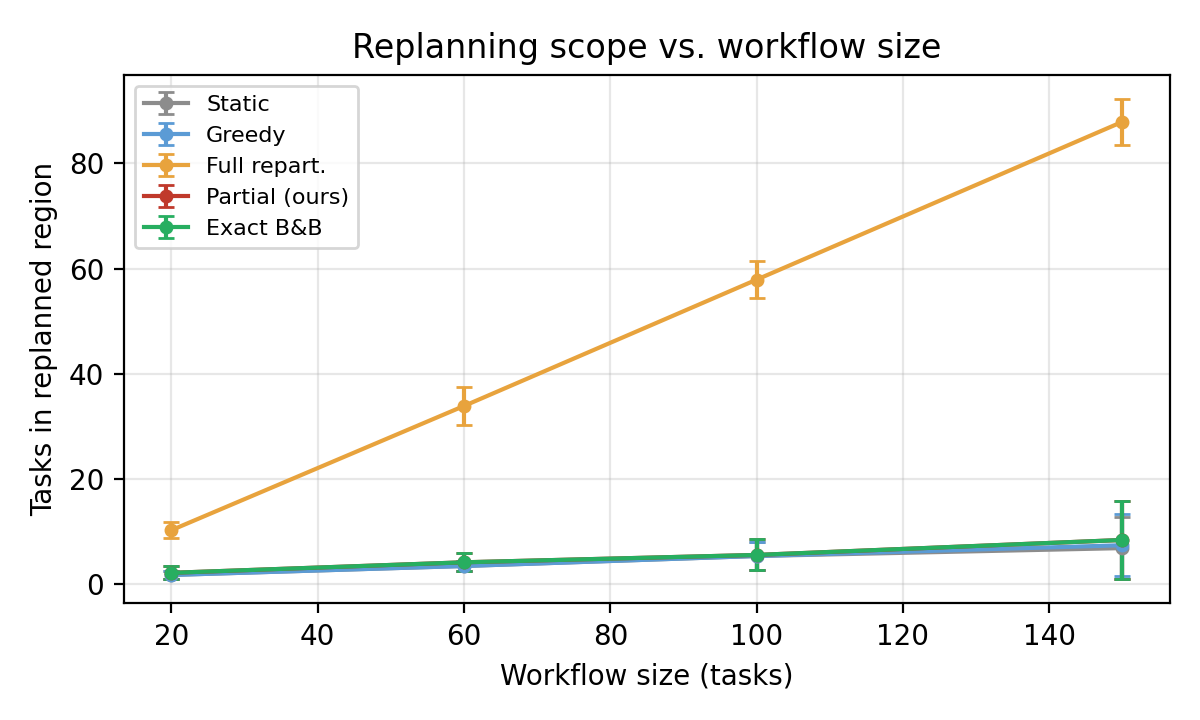
\includegraphics[width=\columnwidth]{../figures/fig4_scale_scope.png}
\caption{Replanning scope vs.\ workflow size. Partial repartitioning stays
proportional to the failure's blast radius; full repartitioning grows
linearly with the workflow.}
\label{fig:scope}
\end{figure}

\begin{figure}[t]
\centering
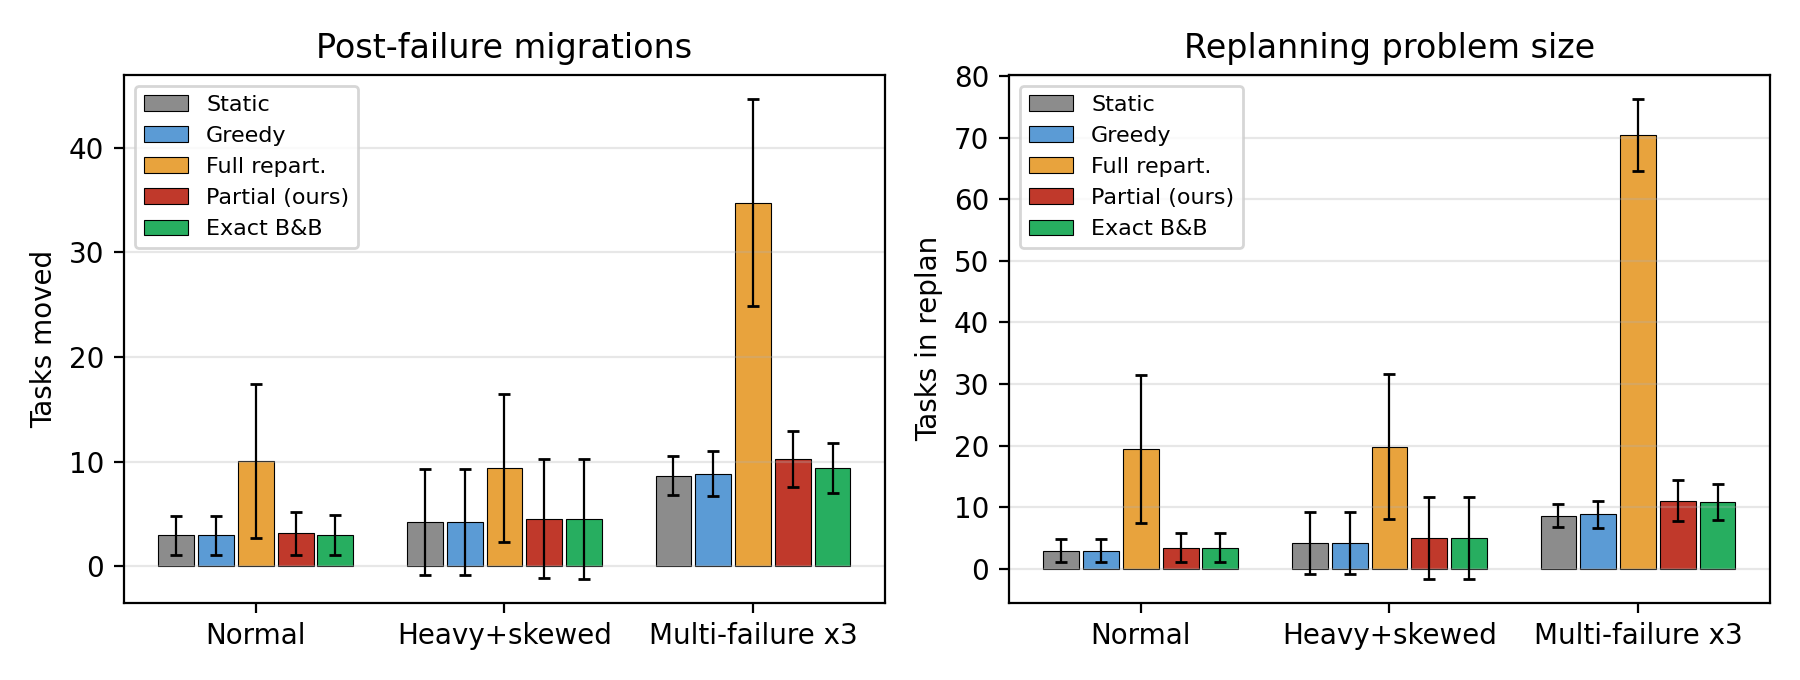
\includegraphics[width=\columnwidth]{../figures/fig2_disruption.png}
\caption{Post-failure disruption: tasks migrated (left) and replanning
problem size (right).}
\label{fig:disruption}
\end{figure}

Table~\ref{tab:normal} summarizes the normal mode. Partial repartitioning
retains 99\% of the exact solver's schedule quality while considering
$\sim$6$\times$ fewer tasks than full repartitioning and moving $\sim$3$\times$
fewer. Communication cost drops an order of magnitude because intact routes
and assignments are preserved.

\begin{table}[t]
\centering
\caption{Normal mode, 120 scenarios (means $\pm$ std)}
\label{tab:normal}
\begin{tabular}{lrrrr}
\toprule
Strategy & Makespan (ms) & Moved & Considered & Comm.\ cost \\
\midrule
static  & 9053 & 3.0 & 3.0  & 13.1 \\
greedy  & 8386 & 3.0 & 3.0  & 13.1 \\
full    & 7762 & 10.1 & 19.5 & 196.9 \\
partial & \textbf{8396} & \textbf{3.1} & \textbf{3.4} & \textbf{19.3} \\
B\&B    & 8386 & 3.0 & 3.4 & 14.2 \\
\bottomrule
\end{tabular}
\end{table}

Under cascaded failures (Table~\ref{tab:multi}) the separation widens:
partial moves 10 tasks and replans 11, versus 35 and 70 for full
repartitioning, and the static fallback meets only 7\% of deadlines.

\begin{table}[t]
\centering
\caption{Multi-failure mode, 3 failures/run, 15 scenarios}
\label{tab:multi}
\begin{tabular}{lrrrrr}
\toprule
Strategy & Makespan (ms) & Moved & Considered & Deadline\% \\
\midrule
static  & 12665 & 8.7 & 8.7 & 7 \\
greedy  & 10558 & 8.8 & 8.8 & 33 \\
full    & 9323  & 34.8 & 70.5 & 62 \\
partial & 10949 & 10.2 & 11.1 & 33 \\
B\&B    & 10600 & 9.4 & 10.9 & 42 \\
\bottomrule
\end{tabular}
\end{table}

\subsection{Optimality validation}

On 28 exported failure instances, the MILP solved to a proven optimum in
under 0.1~s each. Mean gap of the \emph{simulated} makespan to the MILP
subgraph bound: partial 42.4\%, greedy 42.4\%, B\&B 42.6\%, static 48.7\%,
full 29.8\%. This bound excludes post-recovery execution of tasks outside the
affected region, so it is conservative; the tighter same-model comparison is
the exact B\&B solver, against which partial is within 0.1\%.

\subsection{Incremental path repair}

Each failure triggers $\approx 4$ single-source SPT rebuilds on average,
versus a full $10\times10$ all-pairs recompute---corroborating that lazy
repair confines route updates to traffic that actually crosses the failure.

\subsection{Threats to validity}

Greedy ties partial on uniform random workloads: when dependency volume is
low and capacity is homogeneous, per-task placement is already good. The
method's edge appears under data-heavy edges, skewed capacity, and cascaded
failures. The simulator models single-slot execution and no bandwidth
contention; results should be validated on a platform such as
iFogSim~\cite{ifogsim} before deployment claims.

\section{Conclusion}

We presented a dependency-aware partial repartitioning method that recovers
DAG workflows from fog-resource failures by touching only the smallest
consistent affected region, shortlisting replacement resources by
anchor-proximity, penalizing optional movement, and lazily repairing only
affected routes. It recovers with near-optimal schedule quality at a fraction
of the replanning cost of full rescheduling, with the advantage widening
under scale, data-heavy workloads, and cascaded failures. Future work:
hard-deadline-aware placement, bandwidth contention, and online learning of
the boundary-expansion threshold.

\begin{thebibliography}{9}
\bibitem{bhowmick2019}
S.~Bhowmick et al., ``Incremental update of a shortest-path tree on dynamic
graphs,'' \emph{IEEE Trans.}, 2019. doi:10.1109/TBDATA.2019.XXXX (IEEE
Xplore doc.\ 8622042).

\bibitem{DynamicFog}
``Dynamic task distribution in fog computing,'' arXiv:1710.05239, 2017.

\bibitem{DynamicWorkflow}
``Dynamic workflow rescheduling reconsidering unexecutable plan regions,''
\emph{Int.\ J.\ Computational Science and Engineering}, 2011.
doi:10.1504/IJCSE.2011.041219.

\bibitem{UncertainFog}
``Scheduling and rescheduling of tasks under uncertainty in fog systems,''
see related literature.

\bibitem{topcuoglu2002heft}
H.~Topcuoglu, S.~Hariri, and M.-Y. Wu, ``Performance-effective and
low-complexity task scheduling for heterogeneous computing,'' \emph{IEEE
TPDS}, 13(3), 2002.

\bibitem{ifogsim}
H.~Gupta, A.~Vahid Dastjerdi, S.~K. Ghosh, and R.~Buyya, ``iFogSim: A toolkit
for modeling and simulation of resource management techniques in IoT, edge
and fog computing environments,'' \emph{Softw.\ Pract.\ Exp.}, 2017.
\end{thebibliography}

\end{document}
